\chapter{Related Work}
\label{ch:problem-related-work}

A common approach in \acrshort{acr:dtp}, as was discussed in \autoref{ch:introduction}, is to formulate plans by making use of (compact) probabilistic models of the systems under consideration.
In particular we focus our attention to devising \acrshort{acr:mdp} models, which need to accurately define what constitutes the state of the system, reflect uncertainty through transition probabilities, and specify goals through rewards.
The problem we face is that hand-crafting accurate, well-generalizing models is a difficult and time-costly process for a human designer.
To overcome this problem the goal is to automatize the model development process by applying learning algorithms on data that describes the stochastics of the system under consideration.
Therefore this chapter aims to provide some insight into the existing approaches for automating the development of probabilistic models for planning under uncertainty.

First \autoref{sec:learning-state-spaces} gives an overview of the existing algorithms for learning models from execution traces of the system.
Then, in \autoref{sec:active-learning} a number of approaches are examined, which combine offline methods for learning (initial) models with \acrshort{acr:rl} algorithms which update the model parameters online.
Subsequently, \autoref{sec:bayesian-reinforcement-learning} looks into the work that applies a technique known as Bayesian \acrlong{acr:rl} for learning models.

%\section{Problem Formulation}
%\label{sec:problem-formulation}
%
%In \acrshort{acr:dtp} it is common to make use of a (compact) probabilistic model of the environment.
%However, devising an optimal model for a specific system or process can be a daunting and error-prone task, when considering the wide range of possibilities while wanting a compact and computation-cost efficient model.

\section{Learning Probabilistic Models from Execution Traces}
\label{sec:learning-state-spaces}

To facilitate learning system models, the first step is to obtain a dataset which describes the stochastics of the system under consideration.
A common approach of obtaining this data is through the recording of observations made in an exploration phase in which the system aims to gather information about the effect of performing various actions in different situations.
The next step is to learn a probabilistic model which most accurately explains the execution traces obtained in this exploration phase.
In this section a number of these algorithms are considered, where \autoref{sec:baum-welch} evaluates the well-known \textit{Baum-Welch} algorithm that iteratively updates transition and emission probabilities starting from a model with initial estimates of these probabilities, while \autoref{sec:state-merging} addresses a class of algorithms based on merging (time-)states to develop \acrshortpl{acr:mdp}.

\subsection{The Baum-Welch Algorithm}
\label{sec:baum-welch}

The most widely applied approaches for learning probabilistic models are based on maximizing the likelihood of observing the execution traces of the dataset.
When the goal is to learn the parameters of a Markov Chain, the transition probabilities can be estimated as we have seen in \autoref{subsec:markov-chains}, by the ratio of the times a particular transition is observed and the total number of transitions observed from the corresponding starting state.
However, while Markov Chains are similar to \acrshortpl{acr:mdp} in that they describe the evolution of a stochastic process over time, they do not involve decisions on actions to perform.
Due to the close nature of these probabilistic models the likelihood maximization can be applied almost directly to learn the transition probabilities of \acrshortpl{acr:mdp}, although requires more data due to the addition of actions.

In practice, it is more usual to only have a sequence of observations at one's disposal which do not directly map to the states of the system.
The approach of likelihood maximization generalizes to learning partially observable Markov Models through the well-known Baum-Welch algorithm, which is a special instance of the Expectation Maximization (EM) algorithm generally used for learning the parameters of \acrshortpl{acr:hmm}.
Given a discrete or continuous observation space $\mathcal{V}$, a discrete state space $\mathcal{S}$, and a set $\mathcal{O}$ of i.i.d. observation sequences, the algorithm learns a model $\mathcal{M}^\ast = \argmax_\mathcal{M} p(\mathcal{O}\vert\mathcal{M})$.
Informally, this is done by first providing manual estimates of the model parameters and then iteratively computing the expectations of how frequently the transitions and emissions are used (i.e., the \textit{E-step}) and updating these parameters based on those computed expectations (i.e., the \textit{M-step}).
For a more detailed explanation of the Baum-Welch algorithm please refer to the tutorial by \citeauthor{bilmes1998gentle} in \cite{bilmes1998gentle}.

Although the approach turns out to work quite well for learning \acrshortpl{acr:hmm} for recognition purposes, some problems emerge when applying the algorithm to learn \acrshortpl{acr:pomdp} for planning under uncertainty.
That is, the algorithm is well-known to be sensitive to its initialization (particularly in the case of continuous observations) and depending on the choice of the initial model parameters it may result in local maxima.
However, to some extent this problem can be overcome by segmenting the observation sequences using $k$-means clustering to restrict the model to a discrete \acrshort{acr:hmm} or \acrshort{acr:pomdp} (e.g., see \cite{calinon2007learning}).
This discretization however, depending on the choice of the hyper-parameter(s) of the clustering algorithm, might neglect some valuable distinctions between observations or states of the system.

A particularly relevant work is that of \citeauthor{shatkay1997learning} \cite{shatkay1997learning} in which the algorithm is applied to learn \acrshort{acr:pomdp} models in the context of mobile robot navigation.
In their work they make the assumption of a finite set of states whose size is known, and associate each state with a point in some metric space derived from the odometric ability of the robot.
Based on a set of gathered odometric readings an initial \textit{topological} model is learned by applying $k$-means clustering, taking the clusters as the states in which the observations were made, and based on state and observation counts make initial estimates of the model parameters.
Then an adapted version of Baum-Welch is applied which takes into account odometric informaton to iteratively update the model.
The obtained results are compared to those that emerge from the traditional Baum-Welch algorithm, which is used to demonstrate that exploiting odometric information can reduce the number of iterations and improve the final model.

Similarly, an adaptation of the Baum-Welch algorithm is applied in \cite{koenig1996unsupervised} to learn \acrshortpl{acr:pomdp} which exploits prior knowledge of map symmetry and does not adjust probabilities that are assumed to be approximately correct while sensor and actuator models are expected to be similar in different environments.
In this way the amount of required training data is restricted and updating the model happens more selectively and efficiently, although it demands the need for hand-crafting an initial topological model and defining constraints on the model structure.

% Explain drawbacks of Baum-Welch for planning: e.g. local maxima
% https://www.google.nl/url?sa=t&rct=j&q=&esrc=s&source=web&cd=9&cad=rja&uact=8&ved=0ahUKEwiZpvCGmcLTAhXESBQKHTq7Bg0QFghiMAg&url=http%3A%2F%2Fciteseerx.ist.psu.edu%2Fviewdoc%2Fdownload%3Fdoi%3D10.1.1.57.4643%26rep%3Drep1%26type%3Dps&usg=AFQjCNH-b5YR7gExaSuktykOrezijr8kZw&sig2=f4NrRWV0O8dSokuqWWCP7Q
% @techreport{shatkay1997learning,
% title={Learning hidden Markov models with geometric information},
% author={Shatkay, Hagit and Kaelbling, Leslie Pack},
% year={1997},
% institution={Citeseer}
% }

\subsection{State Merging Algorithms}
\label{sec:state-merging}

A completely different class of algorithms is based on the merging of states to acquire probabilistic models.
The type of algorithms that are considered here are based on a method called \textit{Best-First Model Merging} which was first proposed by \citeauthor{stolcke1994best} in \cite{stolcke1994best} to learn \acrshortpl{acr:hmm} for the purpose of speech recognition.

Given a training set $\mathcal{O}$ of i.i.d. observation sequences, this algorithm starts from an initial \acrshort{acr:hmm} whose state-space consists of separate states for each time-step in the sequences.
The entries of the transition and emission matrix are thus initialized with probability one for each of the transitions between subsequent states and each percept in the observation sequence respectively.
Although this \acrshort{acr:hmm} explains the data perfectly it is usually not efficient and therefore the model is iteratively updated by merging those pairs of states that decrease the likelihood the least.
This repeats itself until a stop criterion is reached, which might be when the likelihood falls below a certain value or when a predefined number of states has been reached.

This approach can be adapted for learning \acrshortpl{acr:pomdp} as described in \cite{nikovski1999learning} such that the transition function is initially incomplete as it will only be defined for the actions corresponding to the transitions between subsequent states.
A particular advantage of this approach for planning is that one can choose to adapt the merging criterion so that for instance states are only merged if they both map to the same goal percept.
However, a major disadvantage of the approach is that alternative merges are never considered by the algorithm, although in the end they may result in better models.
This means that the approach is prone to local maxima, although this can be avoided to some extent by considering a set of most promising merges in each iteration, although it would make the algorithm even more cost-expensive than it already is.

A variation of the algorithm is a method seen in \cite{nikovski1999learning} that goes under the name of \textit{State Merging by Trajectory Clustering}, which makes the state merging approach more resilient to \textit{perceptual aliasing}.
In this approach the merging criterion is changed such that in each iteration those pairs of states are merged whose prior and posterior trajectories in the training set are most similar.
The pseudo-code of this method is shown in \autoref{alg:trajectory-clustering} where the similarity of states is thus defined by the length of the trajectories from and towards the states. 
In case of metric observations, one can choose to apply algorithms like $k$-means clustering to cluster the most similar states, or alternatively turn to clustering methods that work on similarity matrices.

\begin{algorithm}
	\caption{State Merging by Trajectory Clustering}
	\label{alg:trajectory-clustering}
	\begin{algorithmic}[1]
		\Require{Training set $\mathcal{O} = \{O_1, \ldots, O_k\}$, Clustering algorithm, hyper-parameter(s) $\theta$, actions $A$}
		\Ensure{\acrshort{acr:mdp} $\mathcal{M} = (\mathcal{S}, s_0, A, \delta, R)$} \Comment{$s_0$ and $R$ are here irrelevant}
		\State Compute similarities of time-states based on trajectories
		\State Cluster most similar time-states to obtain the state-space $\mathcal{S}$
		\State Compute the transition probabilities to obtain $\delta$
		\State \Return \acrshort{acr:mdp} $\mathcal{M}$
	\end{algorithmic}
\end{algorithm}


%One of the main issues faced in learning \acrshort{acr:mdp} models is that of deciding on the state space, while one typically does not know the size of the true state space of the real-world process that generated the training data.
%In fact this state space might even have been continuous, while the state space of the model is typically discrete.
%In particular this might form an issue in the planning phase where a reward function needs to be defined to express the goals in the \acrshort{acr:mdp}, for which there may not be a clear one-to-one mapping from real-world states to model states.

%\blindtext
%
%\subsection{State Merging by Trajectory Clustering}
%\label{sec:trajectory-clustering-merging}
%
%\blindtext


%\showoutline{
%
%\noindent\textbf{Iterative Adjustment of Probabilities}:
%\begin{itemize}
%	\item Likelihood maximization for Markov Chains/MDPs, which generalizes to Baum-Welch for HMMs/POMDPs
%	\item Gradient-Ascent
%\end{itemize}
%
%\begin{figure}[]
%	\centering
%	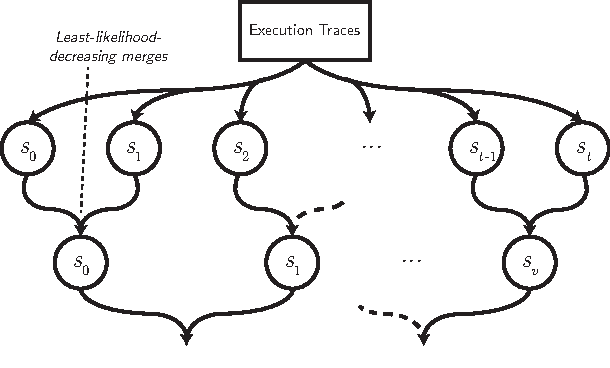
\includegraphics[width=0.8\textwidth]{model-merging-bfmm}
%	\caption{State Merging (Not sure yet whether this should be here)}	% TODO
%	\label{fig:state-merging}
%\end{figure}

%\noindent \textbf{State Merging}:
%\begin{itemize}
%	\item Best-First Model Merging \cite{stolcke1994best}
%	\item State Merging by Trajectory Clustering \cite{nikovski2000learning}
%\end{itemize}
%
%\noindent Other (offline/'data-based') approaches
%
%}

\section{Active (Reinforcement) Learning}
\label{sec:active-learning}

\showoutline{
	\begin{itemize}
		\item Mention Model-Based \acrshort{acr:rl} or Online Model Learning
		\item Refer to approach of combining offline and online planning: using an offline-obtained model and policy, apply model-based \acrshort{acr:rl} to update the parameters \cite{epshteyn2008active}
		\item .....
	\end{itemize}
}

\section{Bayesian Reinforcement Learning}
\label{sec:bayesian-reinforcement-learning}

\showoutline{
\begin{itemize}
	\item Bayesian Inference (see section 2.2.1)
	\item BRL: Maintaining a posterior distribution over possible model parameters
	\item Framework description: \cite{png2011bayesian}
	\begin{itemize}
		\item Initialize distributions over unknown parameters (defining a prior, typically Dirichlet distribution)
		\item Select action based on distributions
		\item Execute action
		\item Observe resulting reward and observation
		\item Update posterior counts of unknown parameters based on observed information
	\end{itemize}
	\item MEDUSA, BEETLE + Other examples?
	\item ..... (To be determined)
\end{itemize}
}

% https://people.eecs.berkeley.edu/~avivt/BRLS_journal.pdf


% TODO;s
%% Fitting Markov Chains/MDPs:
	% Refer back to section 2.2.1:
	% - likelihood maximization
	% - Bayesian inference/optimization
%% Fitting HMMs/POMDPs:
	% ITERATIVE ADJUSTMENT OF PROBABILITIES:
	% - Baum-Welch Algorithm
	% - Gradient-Ascent in Likelihood
	% STATE MERGING
	% - Best-first
	% - Trajectory clustering
%% Reinforcement Learning: Online Model Learning

%% However, most of the previous works assume the state-space of the probabilistic model to be known.

%\section{Bayesian Reinforcement Learning}
%\label{sec:bayesian-reinforcement-learning}

% 

%
%\section{Overview}
%\label{sec:related-work-overview}
%
%% 